% Paste this file into main.tex in Overleaf, then replace the author names.
% Upload the four PNGs named in the figure blocks. They can go in figures/.
\documentclass[11pt,letterpaper]{article}
\usepackage[T1]{fontenc}
\usepackage{lmodern}
\usepackage[margin=0.8in]{geometry}
\usepackage{microtype}
\usepackage{amsmath,amssymb}
\usepackage{graphicx}
\usepackage{booktabs,tabularx,adjustbox}
\usepackage{caption,enumitem,placeins}
\usepackage[hidelinks]{hyperref}

\graphicspath{{figures/}{results/}{../results/}}
\captionsetup{font=small}
\setlist[itemize]{topsep=0.4em,itemsep=0.2em,parsep=0pt}
\setlength{\intextsep}{9pt plus 2pt minus 2pt}
\setlength{\textfloatsep}{12pt plus 3pt minus 3pt}

\title{VAE vs.\ DCGAN: The Fidelity--Diversity Trade-off Under a Shared Architecture\\[0.6em]
  \large COMP 4102 Final Project: comparing two computer vision methods on a dataset}
\author{TEAM MEMBER NAMES}
\date{}

\begin{document}
\maketitle

\section{Problem and motivation}\label{sec:motivation}

A generative image model learns an unknown distribution
\(p_\text{data}(x)\) from examples and then produces new images from it.
Two classic families do this in very different ways. A
\textbf{Variational Autoencoder (VAE)} maximises a lower bound on the
likelihood of the data \cite{kingma2014}. A \textbf{Generative
Adversarial Network (GAN)} trains a generator to fool a learned
discriminator \cite{goodfellow2014}. A common observation is that VAE
samples are \emph{blurry but varied}, while GAN samples are \emph{sharp
but may miss parts of the data} (``mode collapse''). This trade-off
between \textbf{fidelity} (each sample looks real) and
\textbf{diversity} (the samples cover the whole data distribution)
matters in practice: synthetic training data is useless if it is
unrealistic and harmful if it covers only some classes. Measuring the
trade-off is itself a vision problem. A generated image has no
ground-truth target, so the evaluation must compare \emph{distributions}
of images.

Published comparisons usually give each objective its own separately
tuned network, which makes it hard to tell whether a difference comes
from the objective or from the architecture. We therefore ask:
\textbf{with the same image-producing network, latent size, data and
training budget, how do a VAE and a DCGAN trade off fidelity/sharpness
against diversity/mode coverage?} We test three hypotheses on
Fashion-MNIST (3 seeds, plus two ablations):

\begin{itemize}

\item
  \textbf{H1:} the GAN produces sharper samples with a lower FID.
\item
  \textbf{H2:} the VAE covers the data better (higher recall, no mode
  collapse) and trains more stably.
\item
  \textbf{H3:} the VAE has a smoother latent space.
\end{itemize}

\section{Method}\label{sec:method}

\subsection{Variational Autoencoder}\label{sec:vae}

An encoder maps an image \(x\) to the mean \(\mu(x)\) and log-variance
\(\log\sigma^2(x)\) of a Gaussian posterior \(q(z\mid x)\) over a
\(d\)-dimensional latent code. A decoder maps \(z\) back to an image
\(\hat x\), and the prior is \(p(z)=\mathcal N(0,I)\). Training
maximises the evidence lower bound (ELBO) \cite{kingma2014}:

\[\log p(x) \;\ge\; \mathbb E_{q(z\mid x)}\big[\log p(x\mid z)\big] \;-\; \mathrm{KL}\big(q(z\mid x)\,\|\,p(z)\big).\]

We use a Gaussian decoder with fixed variance, so \(-\log p(x\mid z)\)
is the squared error \(\|x-\hat x\|^2\) \textbf{summed over pixels} (up
to a constant). The KL between two Gaussians has a closed form,
\(\tfrac12\sum_j(\mu_j^2+\sigma_j^2-\log\sigma_j^2-1)\). Our loss per
image is therefore

\[\mathcal L_\text{VAE} = \|x-\hat x\|^2 + \beta\,\mathrm{KL}\big(q(z\mid x)\,\|\,\mathcal N(0,I)\big),\]

with \(\beta=1\) for the standard VAE and \(\beta\neq1\) for a
\(\beta\)-VAE \cite{higgins2017}. Sampling inside the network is made
differentiable with the \emph{reparameterization trick},
\(z=\mu+\sigma\odot\varepsilon\) with
\(\varepsilon\sim\mathcal N(0,I)\), so gradients flow through \(\mu\)
and \(\sigma\).

\textbf{Design choice: sum, not mean, over pixels.} A \(32 \times 32\)
image contributes 1024 squared-error terms, while the KL has only
\(d=32\) terms. Averaging the reconstruction error over pixels (a common
shortcut) would make the KL about \(1000\times\) stronger. That is a
hidden \(\beta \approx 1000\), which changes the very blurriness we want
to measure. With the sum, the loss is the true negative ELBO and
\(\beta\) is the only weight on the KL.

\textbf{Why VAEs blur.} For a given \(z\), the decoder output that
minimises expected squared error is the \emph{mean} of all images whose
posteriors overlap at \(z\). The KL term pulls every posterior towards
the same prior, so these posteriors do overlap. The decoder then outputs
an average of several plausible images, for example shirts with
different textures, and averaging acts as a low-pass filter.

\subsection{Deep Convolutional GAN}\label{sec:gan}

A generator \(G\) maps \(z\sim\mathcal N(0,I)\) to an image, and a
discriminator \(D\) outputs the probability that its input is real.
\(D\) minimises binary cross-entropy (real \(\to\) 1, fake \(\to\) 0).
\(G\) minimises the \emph{non-saturating} loss \(-\log D(G(z))\). This
has the same fixed point as the original minimax game but gives stronger
gradients early in training, when \(D\) easily rejects the fakes
\cite{goodfellow2014}. We follow the DCGAN recipe \cite{radford2016}:
strided (transposed) convolutions, batch normalisation, ReLU/LeakyReLU,
\(\mathcal N(0,0.02)\) initialisation, and Adam with learning rate
\(2\cdot10^{-4}\) and \(\beta_1=0.5\). We alternate one \(D\) step and
one \(G\) step.

\textbf{Why GANs are sharp but can drop modes.} \(D\) is itself a CNN
and detects blur easily, so \(G\) is pushed towards crisp, realistic
images. However, \(G\) is only penalised for samples that \emph{look
fake}, never for data it \emph{fails to produce}. Nothing in the
objective asks \(G\) to cover every mode, so mapping many latent codes
to a few convincing images is a stable shortcut (the ``Helvetica
scenario'' in \cite{goodfellow2014}).

\subsection{One architecture for both models (fairness by
construction)}\label{sec:architecture}

The VAE decoder and the GAN generator are the \textbf{same class},
\texttt{ConvDecoder}. Its transposed convolutions grow the image from
\(1 \times 1\) to 4, 8, 16 and 32 pixels with 256/128/64 channels, BN +
ReLU and a tanh output (788k parameters). The VAE encoder and the
discriminator are also one class, \texttt{ConvEncoder}. Its strided
convolutions shrink the image from 32 to 4 pixels with LeakyReLU, and
only its output head differs: \(2d\) numbers (\(\mu\), \(\log\sigma^2\))
for the VAE and one logit for \(D\). Unit tests check that the image
networks are identical and that neither model config overrides a shared
setting (Table~\ref{tab:protocol}).

\begin{table}[!htbp]
\centering
\small
\begin{tabularx}{\linewidth}{@{}*{2}{>{\raggedright\arraybackslash}X}@{}}
\toprule
Shared by both models & Different (and why) \\
\midrule
Data, padding, scaling to \([-1, 1]\) & \textbf{Training objective}: the variable under study \\
Image-producing network (\texttt{ConvDecoder}, 788k params) & Encoder head: 2d outputs (VAE) vs.~1 (D) \\
Latent size \(d=32\), batch size 128, 30 epochs, seeds 0/1/2 & Optimiser settings: each paper's standard (VAE: Adam \(10^{-3}\); DCGAN: Adam \(2\cdot10^{-4}\), \(\beta_1=0.5\)) \\
DCGAN weight initialisation &  \\
Evaluation code, the 10,000 latent vectors, all metrics &  \\
\bottomrule
\end{tabularx}
\caption{Fair-comparison protocol. Shared settings live in one config file (\texttt{configs/shared.yaml}) that both model configs inherit.}
\label{tab:protocol}
\end{table}


\subsection{Evaluation}\label{sec:evaluation}

We compare the \emph{distribution} of 10,000 generated images with the
10,000 Fashion-MNIST test images
(Table~\ref{tab:metrics}) in two feature spaces. The
first is the standard \textbf{Inception-v3} pool features for FID
\cite{heusel2017} (2048-d). The second is the 128-d penultimate layer of
our own \textbf{evaluation CNN} (90.7\% test accuracy), which is trained
only to \emph{measure} the generators. We add it because Inception was
trained on ImageNet photographs, not on \(32 \times 32\) grayscale
clothing.

\begin{table}[!htbp]
\centering
\small
\begin{tabularx}{\linewidth}{@{}p{1.19in}>{\raggedright\arraybackslash}Xl@{}}
\toprule
Metric & What it measures & Better \\
\midrule
FID \cite{heusel2017} & Fréchet distance between Gaussians fitted to real and generated features: fidelity + diversity & \(\downarrow\) \\
Precision / recall \cite{kynkaanniemi2019} & share of generated samples inside the real manifold (fidelity) / of real samples inside the generated manifold (diversity); \(k=3\) nearest-neighbour balls & \(\uparrow\) \\
Modes, class KL & evaluation-CNN labels of the samples: classes with \(\geq 1\%\) of them; KL(\(p_\text{gen}\,\|\,p_\text{real}\)) & \(\uparrow\) / \(\downarrow\) \\
Laplacian var. \cite{pechpacheco2000} & edge strength (2nd-derivative filter) & \(\approx\) real \\
HF ratio & share of 2-D FFT energy above 0.25 cycles/pixel & \(\approx\) real \\
Interp. CV & std/mean of feature-space steps along 100 slerp paths \cite{white2016} of 10 frames; proxy for perceptual path length \cite{karras2019} & \(\downarrow\) \\
NN ratio & median pixel distance generated \(\to\) nearest training image, divided by the same for test images & \(\approx\) 1 \\
Recon. PSNR & VAE only: encoder--decoder reproduction of test images & \(\uparrow\) \\
\bottomrule
\end{tabularx}
\caption{Metrics. The two sharpness metrics are classical CV operations (edge detection and the Fourier transform). Values \emph{above} the real level mean noise, not extra sharpness.}
\label{tab:metrics}
\end{table}


Two checks make these numbers interpretable. First, \textbf{unit tests
on inputs with a known answer}: identical sets give FD = 0; a
``generator'' that produces only one of two clusters gets precision
\textgreater{} 0.95 but recall \(\approx\) 0.5; blurring lowers both
sharpness measures. Second, a \textbf{real-vs-real baseline} runs the
same metric code with 10,000 real \emph{training} images in place of the
generated ones. This gives the best score a perfect generator could
expect with our sample size and feature spaces.

\section{Implementation and data}\label{sec:implementation}

\textbf{Data.} Fashion-MNIST \cite{xiao2017} has 60,000 training and
10,000 test grayscale \(28 \times 28\) images in 10 balanced clothing
classes. We \textbf{zero-pad} the images to \(32 \times 32\) instead of
resizing them, because interpolation would blur the \emph{real} images,
which are the reference for our sharpness metrics. Pixels are scaled to
\([-1, 1]\) to match the tanh output. The models train on the training
split only, and the test split is the reference for every metric.

\textbf{Code.} We wrote the project in PyTorch (commands in
\texttt{README.md}). Every run saves its config, a per-epoch loss log,
sample grids and a checkpoint every 5 epochs. One script evaluates both
models with the same 10,000 latent vectors, so the grids in this report
show the same random draws for both models and are not cherry-picked.
Every table and figure is generated by \texttt{src/analysis.py} from the
saved metrics. For Inception we use the standard FID port in
torchmetrics/torch-fidelity \cite{torchmetrics}. There are 49 automated
tests, including one that runs the whole pipeline end to end on a toy
dataset.

\textbf{Training.} Each model trains for 30 epochs: 468 mini-batches of
128 images per epoch, 14,040 updates in total. We use seeds 0, 1 and 2
on a laptop GPU (Apple silicon, PyTorch MPS). A VAE run takes about 4
minutes and a DCGAN run about 6.5, because the GAN needs two
forward/backward passes per step.

\section{Experiments and results}\label{sec:experiments}

We run four experiments:

\begin{itemize}

\item
  \textbf{E1, main comparison.} VAE vs.~DCGAN at the default settings, 3
  seeds each.
\item
  \textbf{E2, learning curves.} Every saved checkpoint (every 5 epochs)
  of the E1 runs, evaluated with 5,000 samples.
\item
  \textbf{E3, latent size.} \(d\in\{8,32,128\}\) for both models.
\item
  \textbf{E4, KL weight.} \(\beta\in\{0.5,1,4\}\) for the VAE.
\end{itemize}

E3 and E4 use one seed (seed 0); their \(d=32\), \(\beta=1\) entries are
the E1 means.

\subsection{Main comparison (E1)}\label{sec:main}

\begin{table}[!htbp]
\centering
\small
\setlength{\tabcolsep}{3pt}
\begin{adjustbox}{max width=\linewidth}
\begin{tabular}{@{}lcccccccc@{}}
\toprule
Model & FID-Inc \(\downarrow\) & FID-clf \(\downarrow\) & Prec. \(\uparrow\) & Recall \(\uparrow\) & Class KL \(\downarrow\) & Lapl. var & HF ratio & Interp. CV \(\downarrow\) \\
\midrule
VAE & \(56.9 \pm 1.6\) & \(20.7 \pm 1.2\) & \(0.695 \pm 0.008\) & \(0.489 \pm 0.007\) & \(0.22 \pm 0.01\) & \(0.038 \pm 0.001\) & \(0.034 \pm 0.001\) & {\boldmath \(0.51 \pm 0.01\)} \\
DCGAN & {\boldmath \(13.3 \pm 0.5\)} & {\boldmath \(1.29 \pm 0.05\)} & {\boldmath \(0.852 \pm 0.008\)} & {\boldmath \(0.854 \pm 0.001\)} & {\boldmath \(0.022 \pm 0.005\)} & {\boldmath \(0.146 \pm 0.001\)} & {\boldmath \(0.100 \pm 0.004\)} & \(0.69 \pm 0.02\) \\
Real data & 2.40 & 0.034 & 0.903 & 0.893 & 0.005 & 0.150 & 0.104 & -- \\
\bottomrule
\end{tabular}
\end{adjustbox}
\caption{Main results, mean \(\pm\) std over 3 seeds (precision/recall in the classifier space). Last row: the same metrics on 10,000 real training images. Bold = better model. Every run covers all 10 classes.}
\label{tab:main}
\end{table}


\begin{figure}[!htbp]
\centering
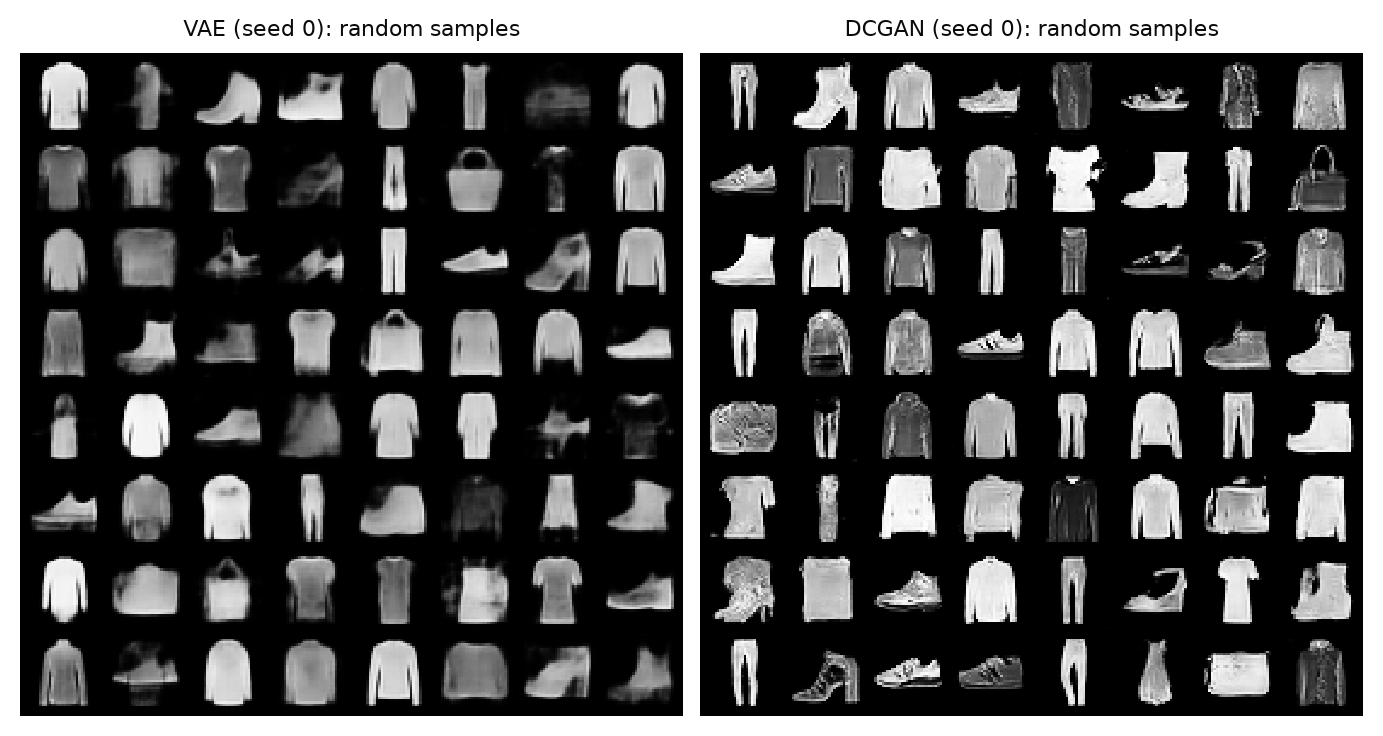
\includegraphics[width=0.68\linewidth]{qualitative_samples.png}
\caption{Random samples from the same latent vectors (not cherry-picked). Left: VAE. Right: DCGAN.}
\label{fig:samples}
\end{figure}

\begin{figure}[!htbp]
\centering
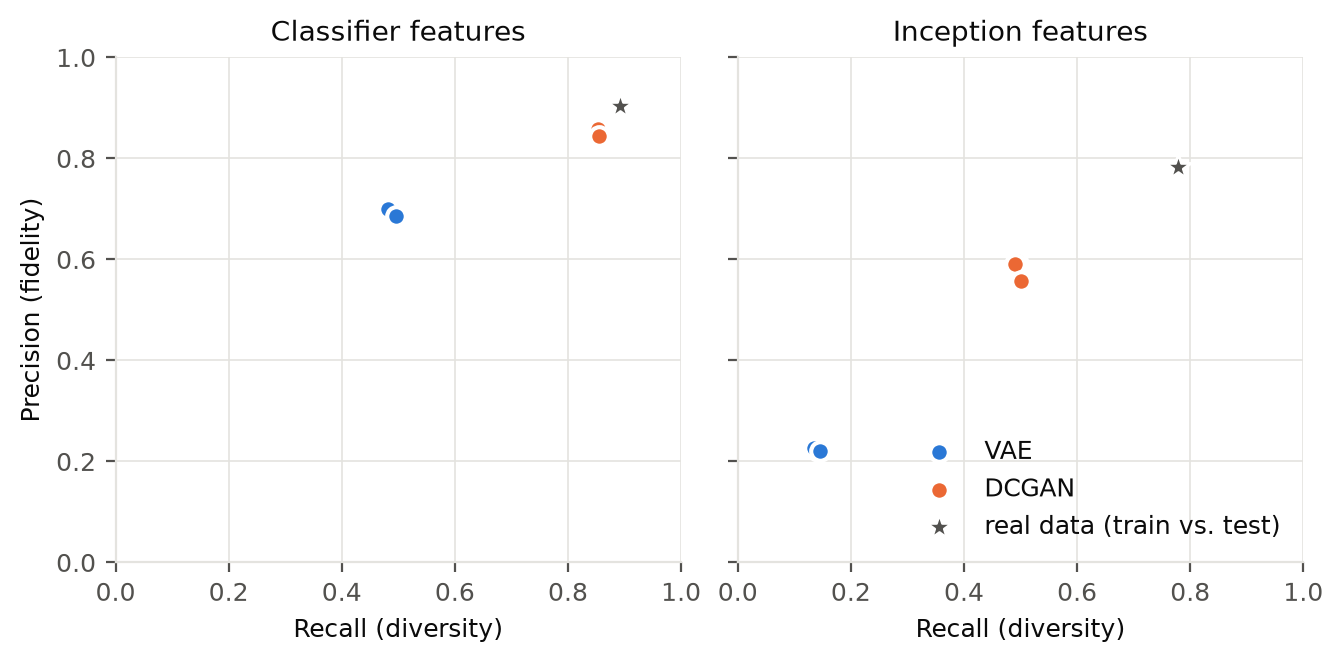
\includegraphics[width=0.67\linewidth]{precision_recall.png}
\caption{Precision vs.~recall: one dot per seed; the star is the real-data baseline.}
\label{fig:precision-recall}
\end{figure}

The DCGAN scores better than the VAE on every metric except
interpolation CV (Table~\ref{tab:main}). Its FID is
\(16\times\) lower in the classifier space (1.29 vs.~20.7) and
\(4\times\) lower in the Inception space (13.3 vs.~56.9). Its precision
and recall (0.85 / 0.85) are close to the real-data baseline (0.90 /
0.89), while the VAE reaches 0.70 precision but only 0.49 recall
(Figure~\ref{fig:precision-recall}). Both models produce
all 10 classes, but the VAE's class distribution is \(10\times\) further
from the real one (KL 0.22 vs.~0.022). The DCGAN's Laplacian variance
and HF ratio are within 4\% of the real images; the VAE keeps about a
quarter of the real edge energy and a third of the high-frequency
energy, visible as blur in Figure~\ref{fig:samples}.

\subsection{Training dynamics (E2)}\label{sec:training}

The DCGAN's FID-clf falls fast until epoch 15 (\(11.3 \to 2.6\)) and
then slowly (1.5 at epoch 30). The VAE improves more slowly and is
\textbf{still improving at epoch 30} (\(22.3 \to 21.1\) over the last 5
epochs; Figure~\ref{fig:learning}). To test whether this
budget is fair, we trained VAE seed 0 for 60 epochs: FID-clf fell only
from 21.1 to 18.4 (recall \(0.49 \to 0.52\), Laplacian variance
\(0.039 \to 0.044\)), closing 14\% of the gap to the DCGAN, so we kept
30 epochs. The min--max bands are narrow for both models, and the
discriminator never overpowered the generator: in every epoch of all
seeds \(D(G(z))\) stayed in {[}0.17, 0.32{]} and \(D(x)\) in {[}0.68,
0.83{]}.

\begin{figure}[!htbp]
\centering
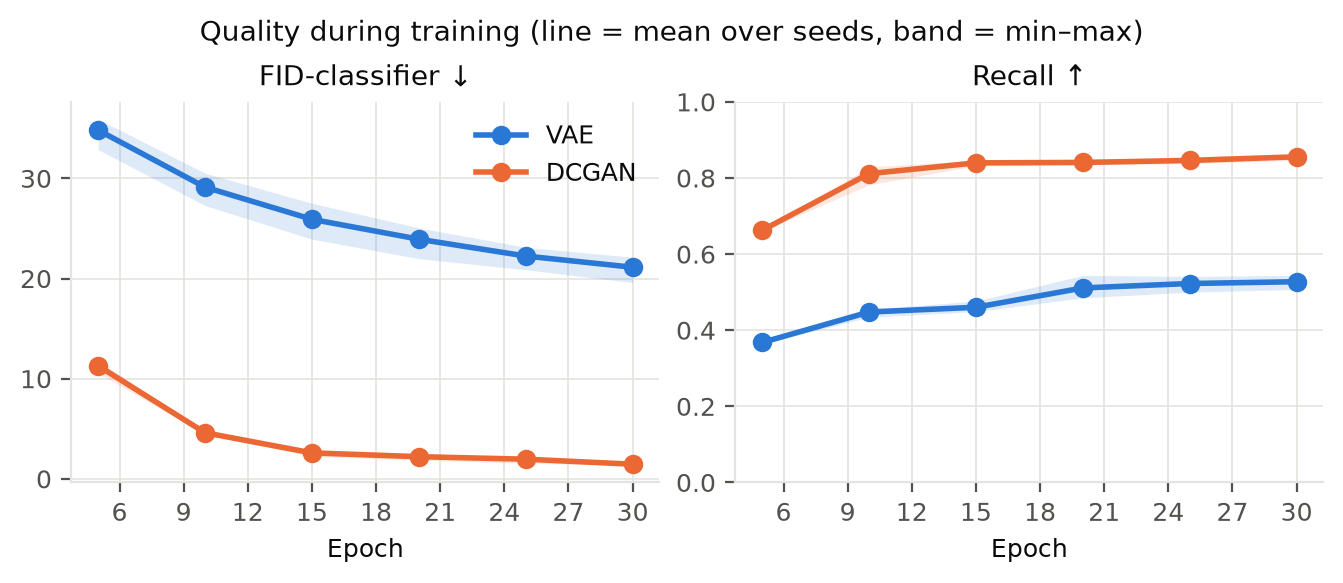
\includegraphics[width=0.72\linewidth]{learning_curve.png}
\caption{FID-classifier (left) and recall (right) during training: mean over seeds, band = min--max. The loss curves are in \texttt{results/training\_curves.png}.}
\label{fig:learning}
\end{figure}

\subsection{Ablations (E3, E4)}\label{sec:ablations}

\begin{table}[!htbp]
\centering
\small
\begin{tabular}{@{}lccc@{}}
\toprule
FID-clf / recall & \(d=8\) & \(d=32\) & \(d=128\) \\
\midrule
VAE & 19.7 / 0.40 & 20.7 / 0.49 & 22.5 / 0.49 \\
DCGAN & 1.19 / 0.82 & 1.29 / 0.85 & 2.04 / 0.85 \\
\bottomrule
\end{tabular}
\caption{Latent-size ablation.}
\label{tab:latent}
\end{table}


\textbf{Latent size (Table~\ref{tab:latent}).} The
ranking never changes. The only clear effect is that \(d=8\) lowers the
VAE's recall (0.40 vs.~0.49) and PSNR (21.3 vs.~22.4 dB); other
differences are within the seed noise of E1.

\begin{table}[!htbp]
\centering
\small
\begin{tabular}{@{}lcccccc@{}}
\toprule
\(\beta\) & FID-clf \(\downarrow\) & Prec. \(\uparrow\) & Recall \(\uparrow\) & Lapl. var & Interp. CV \(\downarrow\) & Recon PSNR \(\uparrow\) \\
\midrule
0.5 & 22.0 & 0.64 & \textbf{0.61} & \textbf{0.041} & \textbf{0.45} & \textbf{23.4} \\
1 & \textbf{20.7} & 0.70 & 0.49 & 0.038 & 0.51 & 22.4 \\
4 & 24.0 & \textbf{0.72} & 0.14 & 0.028 & 0.63 & 20.1 \\
\bottomrule
\end{tabular}
\caption{KL-weight ablation for the VAE (real Laplacian variance: 0.150).}
\label{tab:beta}
\end{table}


\textbf{KL weight (Table~\ref{tab:beta}).} As expected,
a larger \(\beta\) makes the samples blurrier (Laplacian variance
\(0.041 \to 0.028\)) and the reconstructions worse. It also moves the
VAE along the precision--recall trade-off: precision rises slightly
(\(0.64 \to 0.72\)) while recall collapses (\(0.61 \to 0.14\)). Contrary
to our expectation, the latent space did \textbf{not} become smoother:
the interpolation CV rose from 0.45 to 0.63.

\section{Analysis and discussion}\label{sec:discussion}

\textbf{H1: fidelity and sharpness. Supported.} The DCGAN's edge
statistics match the real images (Laplacian variance 0.146 vs.~0.150, HF
ratio 0.100 vs.~0.104) without exceeding them, so its sharpness is real
detail rather than noise. Precision and FID agree in both feature
spaces. This is what \S\ref{sec:method} predicts: the squared-error loss
makes the VAE decoder output a conditional \emph{mean}, which erases any
detail that differs between the plausible images behind a code, whereas
a CNN discriminator easily detects missing high frequencies and pushes
the generator to produce them. E4 confirms the mechanism: a stronger KL
means more averaging and less sharpness.

\textbf{H2: diversity, mode coverage and stability. Not supported},
which is our most interesting result. The DCGAN does not drop modes:
every class makes up 6--13\% of its samples (ideal 10\%), and its recall
is close to the real baseline. The VAE produces all 10 classes but
unevenly: too many pullovers (25\%) and ankle boots (18\%), too few
coats (2\%) and sandals (5\%). These pairs differ mainly in \emph{fine
detail} (a coat is a pullover with a zip; a sandal is an ankle boot with
gaps between the straps), so once blur removes the detail, the
evaluation CNN labels the sample as the plainer class. Blur also
explains the low recall. Recall asks whether each real image lies within
the k-NN ball of some generated sample, and real images defined by
texture or thin structures have no blurry counterpart nearby. In a
learned feature space, blur therefore costs \textbf{diversity as well as
fidelity}. Nor was the GAN less stable: the relative seed-to-seed std of
FID is 3--6\% for both models, and \(D\) never overpowered \(G\)
(\S\ref{sec:training}). Mode collapse simply did not occur on this
balanced dataset with the DCGAN recipe.

\textbf{H3: latent smoothness. Supported, with a caveat.} The VAE's
interpolation steps are more even (CV 0.51 vs.~0.69). In
\texttt{qualitative\_interpolation.png} the VAE paths morph gradually
(trousers widen into a dress), while several DCGAN paths stay almost
constant and then jump in the last frames (a sneaker turns into
trousers). The KL term makes the posteriors of similar images overlap,
so nearby codes decode to similar images; the GAN loss never constrains
what lies \emph{between} two codes. The caveat is E4: a larger \(\beta\)
raised the CV, perhaps because a strong KL switches off most latent
dimensions, so the output barely changes inside a class and then jumps
at a class boundary (one seed, so this remains a hypothesis).

\textbf{Successes and failures.}

\begin{figure}[!htbp]
\centering
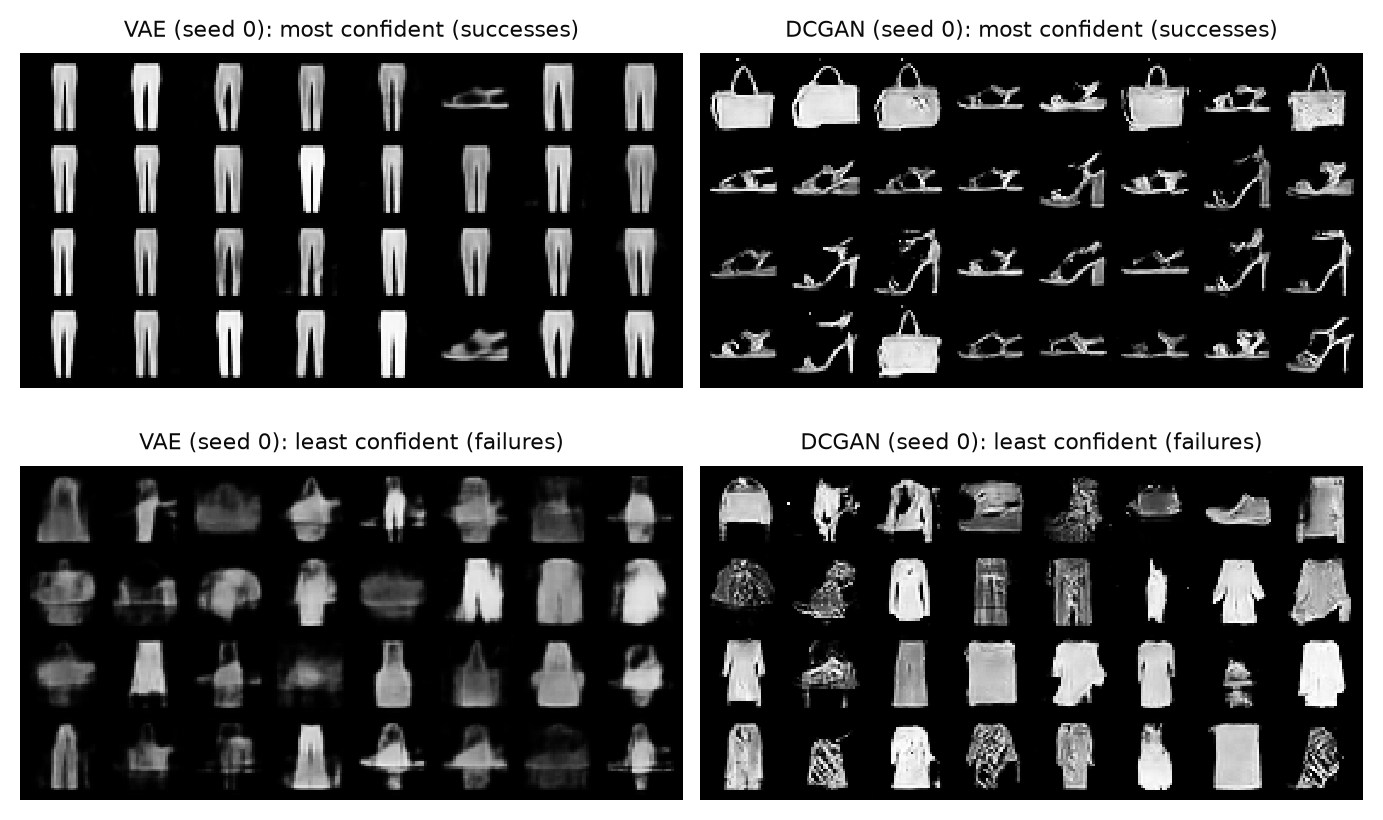
\includegraphics[width=0.68\linewidth]{qualitative_success_failure.png}
\caption{Most (top) and least (bottom) confident samples according to the evaluation classifier.}
\label{fig:success-failure}
\end{figure}

The two models succeed on different classes
(Figure~\ref{fig:success-failure}, top): the VAE on
trousers, whose silhouette survives blur, and the DCGAN on bags and
high-heeled sandals, exactly the fine-structured classes the VAE
under-produces. The VAE's failures are blurry \emph{blends of two
classes} (half shirt, half bag): the averaging of \S\ref{sec:vae} made
visible. The DCGAN's failures are sharp but wrong: high-frequency
texture artefacts and shapes halfway between shirt, dress and coat, with
no repeated items. Neither model copies its training data (NN ratio 1.00
for the VAE, 1.07 for the DCGAN). The \(\beta = 4\) VAE's 0.80 looks
like memorisation, but a blurry average image is simply close in pixel
distance to many training images.

\FloatBarrier

\subsubsection*{Limitations.}

\begin{itemize}

\item
  FID-Inception runs on \(32 \times 32\) grayscale images, far from
  ImageNet; even real-vs-real precision/recall there is only 0.78 (0.90
  with our classifier). Both spaces rank the models the same way, so we
  \textbf{lead with the classifier space} and report FID-Inception for
  comparability.
\item
  The evaluation classifier (90.7\% accuracy) is less confident on
  blurry samples (mean confidence 0.79 VAE, 0.88 DCGAN, 0.93 real), so
  class coverage partly measures blur.
\item
  The VAE was still improving slowly at epoch 30 (\S\ref{sec:training});
  the ablations use one seed; the GAN has no encoder, so reconstruction
  is measured for the VAE only.
\item
  One small architecture and dataset, and untuned paper-default
  optimisers: the results may not transfer to larger models or colour
  images.
\end{itemize}

\section{Conclusion}\label{sec:conclusion}

With the same network, data and budget, the DCGAN beats the VAE on
Fashion-MNIST in fidelity \textbf{and} diversity (FID-clf 1.3 vs.~20.7,
recall 0.85 vs.~0.49); the VAE keeps a smoother latent space and an
encoder. H1 and H3 held, but H2 did not: the GAN never collapsed, and
the VAE's blur cost it coverage as well as sharpness, because in a
learned feature space blur and diversity are not independent. \(\beta\)
moves the VAE along the precision--recall trade-off but, for the values
we tried, never towards the DCGAN. A natural next step is to remove the
blur at its source (a learned decoder variance or a perceptual loss) and
test whether the VAE's recall recovers.

\begin{thebibliography}{99}

\bibitem{kingma2014}
D. P. Kingma, M. Welling. \emph{Auto-Encoding Variational Bayes.} ICLR,
2014.

\bibitem{goodfellow2014}
I. Goodfellow et al.~\emph{Generative Adversarial Nets.} NeurIPS, 2014.

\bibitem{radford2016}
A. Radford, L. Metz, S. Chintala. \emph{Unsupervised Representation
Learning with Deep Convolutional Generative Adversarial Networks.} ICLR,
2016.

\bibitem{higgins2017}
I. Higgins et al.~\emph{\(\beta\)-VAE: Learning Basic Visual Concepts
with a Constrained Variational Framework.} ICLR, 2017.

\bibitem{heusel2017}
M. Heusel et al.~\emph{GANs Trained by a Two Time-Scale Update Rule
Converge to a Local Nash Equilibrium.} NeurIPS, 2017.

\bibitem{kynkaanniemi2019}
T. Kynkäänniemi et al.~\emph{Improved Precision and Recall Metric for
Assessing Generative Models.} NeurIPS, 2019.

\bibitem{pechpacheco2000}
J. L. Pech-Pacheco et al.~\emph{Diatom Autofocusing in Brightfield
Microscopy: A Comparative Study.} ICPR, 2000.

\bibitem{white2016}
T. White. \emph{Sampling Generative Networks.} arXiv:1609.04468, 2016.

\bibitem{karras2019}
T. Karras, S. Laine, T. Aila. \emph{A Style-Based Generator Architecture
for Generative Adversarial Networks.} CVPR, 2019.

\bibitem{xiao2017}
H. Xiao, K. Rasul, R. Vollgraf. \emph{Fashion-MNIST: a Novel Image
Dataset for Benchmarking Machine Learning Algorithms.} arXiv:1708.07747,
2017.

\bibitem{torchmetrics}
N. Detlefsen et al.~\emph{TorchMetrics: Measuring Reproducibility in
PyTorch.} JOSS, 2022; A. Obukhov et al.~\emph{torch-fidelity}, 2020.

\end{thebibliography}
\end{document}
